% SC4012 --- Chapter 7: Malware Analysis, Sandbox and Attestation (0->100 ground-up)
\chapter{Malware Analysis, Sandboxing and Attestation}
\label{ch:malware}

\begin{quote}
\emph{``Know your enemy as you know your code.''} --- Malware is software with an adversarial goal. We learn how it hides, how we dissect it safely, and how hardware can attest what actually ran.
\end{quote}

\noindent\fbox{\parbox{\dimexpr\linewidth-2\fboxsep-2\fboxrule}{%
\textbf{From zero: what malware wants.} We start from a program that does something the user did not intend (steal, ransom, persist), then see static and dynamic analysis, isolation via sandboxing, and attestation that proves a machine's state to a remote verifier.}}
\vspace{0.4em}

\section*{Learning Outcomes}
After this chapter you will be able to:
\begin{enumerate}[label=(L\arabic*)]
    \item classify malware by behaviour (virus, worm, trojan, ransomware, rootkit) and goal;
    \item apply static (signatures, strings, CFG) and dynamic (sandbox trace) analysis;
    \item explain sandboxing (seccomp, containers, VMs) and its escape surface;
    \item describe remote attestation (TPM, SGX, measured boot) and what it proves;
    \item reason about evasion (packing, anti-VM, polymorphism) and layered detection.
\end{enumerate}

% ============================================================
\section{What Malware Does}
\label{sec:malware-types}
Malware is defined by intent, not by bug: it is software that acts against the user's interest. Behaviour gives the taxonomy: virus (infects hosts), worm (self-propagates over network), trojan (masquerades as benign), ransomware (encrypts for ransom), spyware, rootkit (hides its presence by hooking the OS).

\begin{definition}[Malware]
\emph{Malware} is code that, when executed, violates the user's security policy: exfiltration, persistence, propagation, or denial. \emph{Payload} is the malicious effect; \emph{packer/crypter} is the obfuscation that hides it; \emph{C2} (command-and-control) is the remote infrastructure that directs it.
\end{definition}

\begin{figure}[h]\centering
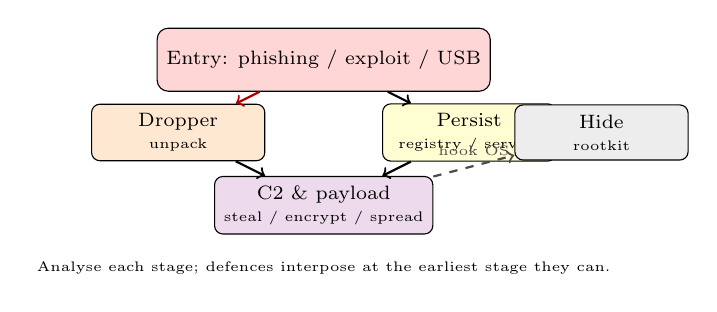
\begin{tikzpicture}[scale=0.84,every node/.style={font=\scriptsize}]
  \node[draw,fill=red!16,rounded corners=4pt,minimum width=2.8cm,minimum height=0.8cm,align=center] (entry) at (0,2.6) {Entry: phishing / exploit / USB};
  \node[draw,fill=orange!18,rounded corners=3pt,minimum width=2.2cm,minimum height=0.7cm,align=center] (drop) at (-2.2,1.5) {Dropper\\ \tiny unpack};
  \node[draw,fill=yellow!18,rounded corners=3pt,minimum width=2.2cm,minimum height=0.7cm,align=center] (persist) at (2.2,1.5) {Persist\\ \tiny registry / service};
  \node[draw,fill=violet!14,rounded corners=3pt,minimum width=2.2cm,minimum height=0.7cm,align=center] (c2) at (0,0.4) {C2 \& payload\\ \tiny steal / encrypt / spread};
  \node[draw,fill=gray!14,rounded corners=3pt,minimum width=2.2cm,minimum height=0.7cm,align=center] (hide) at (4.2,1.5) {Hide\\ \tiny rootkit};
  \draw[->,thick,red!70!black] (entry) -- (drop);
  \draw[->,thick] (entry) -- (persist);
  \draw[->,thick] (drop) -- (c2); \draw[->,thick] (persist) -- (c2);
  \draw[->,thick,dashed,gray!60!black] (c2) -- (hide) node[midway,above,font=\tiny] {hook OS};
  \node[font=\tiny,align=center] at (0,-0.55) {Analyse each stage; defences interpose at the earliest stage they can.};
\end{tikzpicture}
\caption{Malware lifecycle. Entry exploits a human or software flaw; the dropper unpacks the payload; persistence survives reboot; C2 directs the objective; hiding delays detection.}
\label{fig:malware-lifecycle}
\end{figure}

Modern malware is modular: an initial access broker sells entry, a loader fetches the next stage, and the final payload is rented as a service. Defence must therefore work at every stage, not just at the final payload.

% ============================================================
\section{Analysis: Static and Dynamic}
\label{sec:analysis}
\emph{Static analysis} examines the binary without running it: strings, imports, entropy (packed sections have high entropy), control-flow graph, and YARA signatures (byte/regex rules). It is safe and fast but brittle against packing and polymorphism.

\emph{Dynamic analysis} runs the sample in an instrumented environment and records behaviour: syscalls, file/network activity, registry changes. It sees unpacked code but can be evaded if the sample detects the analysis environment.

\begin{lstlisting}[language=Python]
# YARA rule (signature for a family)
rule Emotet_Dropper {
    meta: description = "Emotet dropper heuristic"
    strings:
        $a = "powershell -enc" ascii
        $b = { 4D 5A 90 00 }  // MZ header dropped to disk
        $c = "VirtualAlloc" ascii
    condition: 2 of ($a,$b,$c)
}
# yara -r emotet.yar samples/
\end{lstlisting}

\begin{figure}[h]\centering
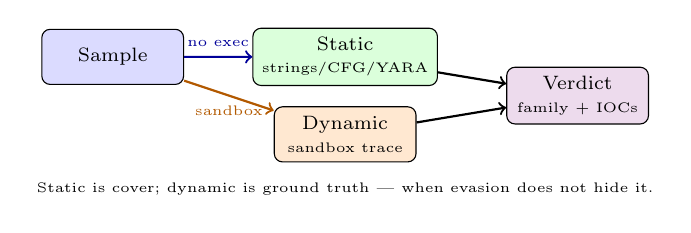
\begin{tikzpicture}[scale=0.82,every node/.style={font=\scriptsize}]
  \node[draw,fill=blue!14,rounded corners=3pt,minimum width=1.8cm,minimum height=0.7cm,align=center] (sample) at (-3.6,1.2) {Sample};
  \node[draw,fill=green!14,rounded corners=3pt,minimum width=1.8cm,minimum height=0.7cm,align=center] (static) at (0,1.2) {Static\\ \tiny strings/CFG/YARA};
  \node[draw,fill=orange!18,rounded corners=3pt,minimum width=1.8cm,minimum height=0.7cm,align=center] (dynamic) at (0,0) {Dynamic\\ \tiny sandbox trace};
  \node[draw,fill=violet!14,rounded corners=3pt,minimum width=1.8cm,minimum height=0.7cm,align=center] (verdict) at (3.6,0.6) {Verdict\\ \tiny family + IOCs};
  \draw[->,thick,blue!60!black] (sample) -- (static) node[midway,above,font=\tiny] {no exec};
  \draw[->,thick,orange!70!black] (sample) -- (dynamic) node[midway,below,font=\tiny] {sandbox};
  \draw[->,thick] (static) -- (verdict); \draw[->,thick] (dynamic) -- (verdict);
  \node[font=\tiny,align=center] at (0,-0.85) {Static is cover; dynamic is ground truth --- when evasion does not hide it.};
\end{tikzpicture}
\caption{Two complementary lenses. Static is fast and misses packed/obfuscated code; dynamic sees real behaviour but can be evaded by environment checks.}
\label{fig:static-dynamic}
\end{figure}

\begin{lstlisting}[language=Python]
# Dynamic trace sketch: syscall log from sandbox (e.g., Cuckoo, CAPE)
trace = [
    ("CreateFile", r"C:\Temp\evil.bin", "WRITE"),
    ("RegSetValue", r"HKCU\Software\Microsoft\Windows\CurrentVersion\Run", "evil"),
    ("Connect", "198.51.100.7:443"),
]
# Rule: file drop + persistence + C2 within 5 sec => high confidence malware
if any("Run" in k for k,_ in trace) and any("Connect"==a for a,_,_ in trace):
    print("suspicious: persistence + C2")
\end{lstlisting}

Evasion catalogue (longer): packing (UPX, custom), polymorphism/metamorphism (re-encrypt or rewrite each copy), anti-VM (check \texttt{VBox}, few files, no mouse movement), anti-debug (\texttt{IsDebuggerPresent}, timing checks), delayed execution, process hollowing (replace a suspended legitimate process), and living-off-the-land (use \texttt{powershell}, \texttt{wmic}, \texttt{mshta} instead of custom code). Behavioural detection thus monitors \emph{actions}, not just \emph{bytes}.

 packing (UPX, custom), polymorphism/metamorphism (re-encrypt or rewrite each copy), anti-VM (check for \texttt{VBox}, few files, no mouse movement), delayed execution, and living-off-the-land (use \texttt{powershell}, \texttt{wmic} instead of custom code).

% ============================================================
\section{Sandboxing: Isolation that Contains}
\label{sec:sandbox}
A sandbox confines untrusted code so that even if it is malicious, its reach is limited. Mechanisms form a hierarchy of strength vs.\ cost.

\begin{description}[leftmargin=1.2em,itemsep=0.35em]
    \item[Seccomp / pledge / Capsicum] Kernel filters that allow-list syscalls or capabilities. Cheap, fine-grained; protects the host from a compromised process.
    \item[Containers (namespaces, cgroups)] Isolate filesystem, network and PIDs but share the kernel; escape via kernel bug is still possible.
    \item[VMs / microVMs (KVM, Firecracker)] Hardware virtualisation gives a separate kernel; stronger isolation, higher startup cost.
\end{description}

\begin{figure}[h]\centering
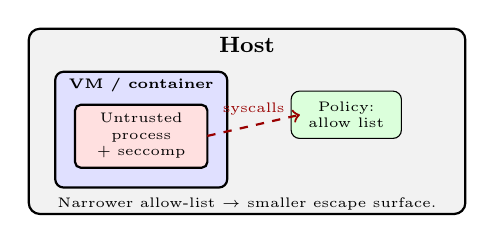
\begin{tikzpicture}[scale=0.84,every node/.style={font=\scriptsize}]
  \draw[thick,fill=gray!10,rounded corners=4pt] (0,0) rectangle (6.6,2.8);
  \node[font=\footnotesize\bfseries] at (3.3,2.55) {Host};
  \draw[thick,fill=blue!12,rounded corners=3pt] (0.4,0.4) rectangle (3.0,2.15);
  \node[font=\tiny\bfseries] at (1.7,1.95) {VM / container};
  \draw[thick,fill=red!12,rounded corners=2pt] (0.7,0.7) rectangle (2.7,1.65);
  \node[font=\tiny,align=center] at (1.7,1.18) {Untrusted\\process\\+ seccomp};
  \node[draw,fill=green!14,rounded corners=3pt,minimum width=1.4cm,minimum height=0.6cm,align=center,font=\tiny] at (4.8,1.5) {Policy:\\allow list};
  \draw[->,thick,red!60!black,dashed] (2.7,1.18) -- (4.1,1.5) node[midway,above,font=\tiny] {syscalls};
  \node[font=\tiny,align=center] at (3.3,0.15) {Narrower allow-list $\to$ smaller escape surface.};
\end{tikzpicture}
\caption{Nested isolation. The untrusted process is restricted by a syscall filter inside a container/VM inside the host. Each layer shrinks the reachable kernel and host surface.}
\label{fig:sandbox-nesting}
\end{figure}

A sandbox is a policy: enumerate what the program \emph{needs} (e.g., \texttt{read}, \texttt{write}, \texttt{openat} on its directory) and deny the rest. Tools: \texttt{seccomp-bpf} on Linux, \texttt{pledge} on OpenBSD, AppArmor/SELinux MAC, gVisor, Firecracker microVMs.

Sandbox escapes are bugs in the policy or in the kernel: overly broad \texttt{openat} that allows \texttt{/etc/shadow}, unfiltered \texttt{ioctl} that reaches a driver, or a kernel use-after-free that the sandbox was supposed to contain. Hence the nesting principle: even if seccomp is bypassed, the container still restricts the filesystem; even if the container is escaped, the VM still isolates the host.

\begin{lstlisting}[language=C]
// seccomp-bpf sketch: allow only read/write/exit (illustrative)
#include <seccomp.h>
void lockdown(void){
    scmp_filter_ctx ctx = seccomp_init(SCMP_ACT_KILL);
    seccomp_rule_add(ctx, SCMP_ACT_ALLOW, SCMP_SYS(read), 0);
    seccomp_rule_add(ctx, SCMP_ACT_ALLOW, SCMP_SYS(write), 0);
    seccomp_rule_add(ctx, SCMP_ACT_ALLOW, SCMP_SYS(exit_group), 0);
    seccomp_load(ctx);
}
\end{lstlisting}

% ============================================================
\section{Attestation: Proving What Ran}
\label{sec:attestation}
Sandboxing limits what \emph{can} happen; attestation proves what \emph{did} happen to a remote party. A Trusted Platform Module (TPM) or TEE (Intel SGX, AMD SEV, ARM CCA) measures boot and code and signs the measurement.

{\sloppy
\begin{definition}[Remote attestation]
A prover with a hardware root of trust produces a \emph{quote}: $\text{Sign}_{sk_{hw}}(\text{measurements} \Vert \text{nonce})$ where measurements are hashes of firmware, bootloader, kernel and application. A verifier checks the signature with the manufacturer's public key and decides whether the measurements match a known-good allow-list.
\end{definition}
\par}

{\sloppy
Measured boot chains hashes: firmware measures bootloader, bootloader measures kernel, kernel measures app; each extends a Platform Configuration Register (PCR) via $PCR_{new}=H(PCR_{old}\Vert \text{measure})$. A single bit change in any stage changes the final PCR, so the quote binds the entire stack.
\par}

Use cases: cloud nodes proving they run the expected enclave to a tenant, IoT devices proving firmware integrity to a fleet manager, and DRM / key management where a key is released only to an attested TEE (sealing). Remote attestation also underpins confidential computing: the customer verifies the cloud's TEE before sending sensitive data.


\begin{remark}[Confidential computing reality]
Attestation proves the TEE is genuine and the measurement matches, but the TCB is large (firmware, microcode, SDK) and side channels (Spectre, L1TF, Plundervolt) have repeatedly breached SGX enclaves. Production use thus pairs attestation with constant-time code inside the enclave, microcode updates, and a fallback that treats TEE compromise as a detectable, attestable failure rather than an impossibility.

\end{remark}

\begin{remark}[What attestation does not do]
It proves \emph{integrity} (what ran), not \emph{absence of bugs} in what ran, nor privacy of data inside the TEE against side channels (SGX has had many). Pair attestation with verification (Ch.~6), sandboxing, and side-channel hardening.
\end{remark}

% ============================================================
\section{Detection at Scale}
\label{sec:detection-scale}
Endpoints stream telemetry (syscalls, ETW, eBPF) to a detector that scores behaviour against rules and ML models. Trade-offs dominate: a sensitive rule (``any PowerShell with -enc'') catches Emotet but fires on admin scripts; a specific rule (YARA with 3/3 strings) is quiet but misses variants. Deploy in tiers: high-precision rules block, medium-precision alert, low-precision log for hunting. Threat intelligence (IOCs, TTPs) and allow-lists tune the layers.

\begin{remark}[Supply-chain lens]
Modern malware often arrives via a compromised dependency or update (SolarWinds, 2020). Attestation (\S\\ref{sec:attestation}) plus reproducible builds and Sigstore signing let a verifier check that the binary it runs matches the source it audited. No single control stops supply-chain compromise; the chain must be measured end to end.
\end{remark}

\begin{remark}[Hunting, not just blocking]
Beyond blocking known families, hunt for TTPs (techniques, tactics, procedures) in the MITRE ATT\&CK matrix: ``process hollowing + registry persistence + DNS tunneling'' is suspicious even if no hash matches. Hunting queries over telemetry catch novel variants that signatures miss.
\end{remark}

{\sloppy
\begin{example}[Living off the land]
An attacker who runs \texttt{powershell -enc} or \texttt{rundll32} with a \texttt{javascript:} payload leaves no custom binary on disk; detection must trigger on the \emph{behaviour} (encoded PowerShell plus network connect) rather than a file hash. This is why behavioural rules and parent-process anomalies matter.
\end{example}
\par}

% ============================================================
\section{Exercises}
\label{sec:ch07-exercises}
{\sloppy
\begin{enumerate}[label=E7.\arabic*, leftmargin=*, itemsep=0.6em]
    \item \textbf{Static triage.} A binary has high-entropy section \texttt{.packed}, imports only \texttt{LoadLibrary} and \texttt{GetProcAddress}, and strings contain \texttt{powershell -enc}. What do you infer? Write a YARA rule and describe how you would unpack it for further static analysis.
    \item \textbf{Dynamic evasion.} A sample checks \texttt{CPUID} hypervisor bit, counts files in \texttt{C:\textbackslash}, and sleeps 10 minutes before contacting C2. How does each evade a sandbox, and what sandbox countermeasures (e.g., VM hardening, time acceleration, network simulation) help?
    \item \textbf{Sandbox policy.} A PDF renderer needs to read one file, render it, and write a PNG. Write a seccomp allow-list for it and argue why \texttt{execve}, \texttt{socket} and \texttt{ptrace} must be denied. What remains as the escape surface?
    \item \textbf{Measured boot chain.} Firmware $F$, bootloader $B$, kernel $K$ are measured as $PCR_{i+1}=H(PCR_i\Vert H(\text{component}))$. Show that changing any byte of $B$ changes the final PCR that the verifier checks, and why replaying an old quote with a fresh nonce fails.
    \item \textbf{Layered defence.} Design detection at three stages (delivery, execution, C2) for a ransomware family: a mail filter, a sandbox rule, and a network indicator. Explain how each stage's false-positive cost shapes its threshold.
\end{enumerate}
\par}

\section*{Chapter Notes}
Malware analysis in Sikorski \& Honig, \emph{Practical Malware Analysis}; YARA by Victor Alvarez. Sandboxing: seccomp-bpf (Drewry, 2012), gVisor, Firecracker (AWS, 2018). Virtualization and containers surveyed in Brenner et al. Attestation from TPM 2.0 spec (TCG) and SGX (McKeen et al., 2013); measured boot and IMA in Sailer et al. (2004). Side-channel limits of TEEs in van Bulck et al.~(Foreshadow, 2018).

% End of Chapter 7
